\documentclass{article}
\usepackage{graphicx} % Required for inserting images
\usepackage{enumitem}
\usepackage{amsmath}
\usepackage{amsfonts}
\usepackage{amssymb}
\usepackage{amstext}
\usepackage{mdframed}
\usepackage{hyperref}
\usepackage{multicol}
\usepackage{comment}
\usepackage{float}
\usepackage{listings}
\usepackage{subcaption}
\hypersetup{
    colorlinks=true,
    linkcolor=darkblue,
    filecolor=magenta,      
    urlcolor=blue,
    citecolor=violet,
    pdftitle={Overleaf Example},
    pdfpagemode=FullScreen,
}
\lstset{
  basicstyle=\ttfamily,
  columns=fullflexible,
}
\usepackage{bbm}
\usepackage[top = 1.5cm, left = 2cm, right = 2cm, bottom = 2cm]{geometry}
\setlength{\parindent}{0 in}
\setlength{\parskip}{0.1 in}

% \graphicspath{ {./Images/} }

% Use this only for rational_quadratic captions/labels
\newcommand{\figrowescaped}[3]{%
  \begin{figure}[htbp]
    \centering
    \begin{subfigure}[b]{0.3\textwidth}
      \includegraphics[width=\textwidth]{Task-02/true_function_#3_n#2_#1.png}
      \caption{True Function}
    \end{subfigure}
    \begin{subfigure}[b]{0.3\textwidth}
      \includegraphics[width=\textwidth]{Task-02/gp_mean_#3_n#2_#1.png}
      \caption{Predicted Mean}
    \end{subfigure}
    \begin{subfigure}[b]{0.3\textwidth}
      \includegraphics[width=\textwidth]{Task-02/gp_std_#3_n#2_#1.png}
      \caption{Predicted Std Dev}
    \end{subfigure}
    \caption{Kernel: rational\_quadratic, Acquisition: #1, Samples: #2}
    \label{fig:#1_#2_rational_quadratic}
  \end{figure}
}

% Normal version for rbf and matern
\newcommand{\figrow}[3]{%
  \begin{figure}[htbp]
    \centering
    \begin{subfigure}[b]{0.3\textwidth}
      \includegraphics[width=\textwidth]{Task-02/true_function_#3_n#2_#1.png}
      \caption{True Function}
    \end{subfigure}
    \begin{subfigure}[b]{0.3\textwidth}
      \includegraphics[width=\textwidth]{Task-02/gp_mean_#3_n#2_#1.png}
      \caption{Predicted Mean}
    \end{subfigure}
    \begin{subfigure}[b]{0.3\textwidth}
      \includegraphics[width=\textwidth]{Task-02/gp_std_#3_n#2_#1.png}
      \caption{Predicted Std Dev}
    \end{subfigure}
    \caption{Kernel: #3, Acquisition: #1, Samples: #2}
    \label{fig:#1_#2_#3}
  \end{figure}
}

\title{Advanced Machine Unlearning: Programming Assignment 4}
\author{Tejas Sharma, Muskaan Jain, Ojas Maheshwari}
\date{Spring 2025}

\begin{document}
\maketitle
\section{Task 0: Environment Setup and Result Reproduction}
\begin{lstlisting}
Using device: mps

--- Model Architecture ---
EnergyRegressor(
    (net): Sequential(
    (0): Linear(in_features=784, out_features=4096, bias=True)
    (1): ReLU(inplace=True)
    (2): Linear(in_features=4096, out_features=2048, bias=True)
    (3): ReLU(inplace=True)
    (4): Linear(in_features=2048, out_features=1024, bias=True)
    (5): ReLU(inplace=True)
    (6): Linear(in_features=1024, out_features=512, bias=True)
    (7): ReLU(inplace=True)
    (8): Linear(in_features=512, out_features=256, bias=True)
    (9): ReLU(inplace=True)
    (10): Linear(in_features=256, out_features=128, bias=True)
    (11): ReLU(inplace=True)
    (12): Linear(in_features=128, out_features=64, bias=True)
    (13): ReLU(inplace=True)
    (14): Linear(in_features=64, out_features=32, bias=True)
    (15): ReLU(inplace=True)
    (16): Linear(in_features=32, out_features=16, bias=True)
    (17): ReLU(inplace=True)
    (18): Linear(in_features=16, out_features=8, bias=True)
    (19): ReLU(inplace=True)
    (20): Linear(in_features=8, out_features=4, bias=True)
    (21): ReLU(inplace=True)
    (22): Linear(in_features=4, out_features=2, bias=True)
    (23): ReLU(inplace=True)
    (24): Linear(in_features=2, out_features=1, bias=True)
    )
)
------------------------

Loading dataset from ./A4_test_data.pt...
Dataset loaded in 0.18s. Shape: x=torch.Size([100000, 784]), energy=torch.Size([100000, 1])
Using device: mps
Using device: mps

--- Test Results ---
Loss: 288.1554
--- Script Finished ---
\end{lstlisting}
We set \texttt{DATASET\_PATH=`./A4\_test\_data.pt'} and loaded the state dictionary of the \texttt{EnergyRegressor} model from \texttt{MODEL\_WEIGHTS\_PATH=`./trained\_model\_weights.pth'}. Above is the output on running \texttt{get\_results.py}.

The files \texttt{A4\_test\_data.pt} and \texttt{trained\_model\_weights.pth} are downloaded from the assignment drive link, and pasted into the directory containing the python script \texttt{get\_results.py}.

\section{Task 1: MCMC Sampling Implementation}
We imported from the task 0 file \texttt{get\_results.py}, the \texttt{EnergyRegressor} class. We also used the \texttt{TSNE} class from \texttt{sklearn.manifold} to visualize the samples generated by the MCMC sampling algorithm that we implemented. Lastly, we imported the \texttt{clock\_gettime} function from the \texttt{time} library to measure the time taken by our sampling algorithms. The file for task 1 is \texttt{sampling\_algos.py}.

We assume that this file is in the same directory as the task 0 file and also has the trained model weights file. On executing this file, we got the following output:
\begin{lstlisting}
Using device: mps
--- Sampling Times ---
Algo-1 Burn-in Time: 26.6275 seconds
Algo-1 Completion Time: 48.6032 seconds
Algo-2 Burn-in Time: 10.4676 seconds
Algo-2 Completion Time: 21.3794 seconds
\end{lstlisting}

We found that the best results were obtained on setting the value of burn-in to 1000 (1000 samples pre-generated before actual sampling), and 1000 samples were generated after that, which were plotted. The value of $\tau$ or the learning rate is set to 0.01.

The above results were generated using these hyperparameters. It is evident that the second algorithm is more than twice as fast as the first, which is understandable considering that we do not evaluate any function (probabilistic) that decides whether we reject or accept the new sample.

\subsection{2D and 3D visualization of generated samples}
\begin{figure}[H]
    \centering
    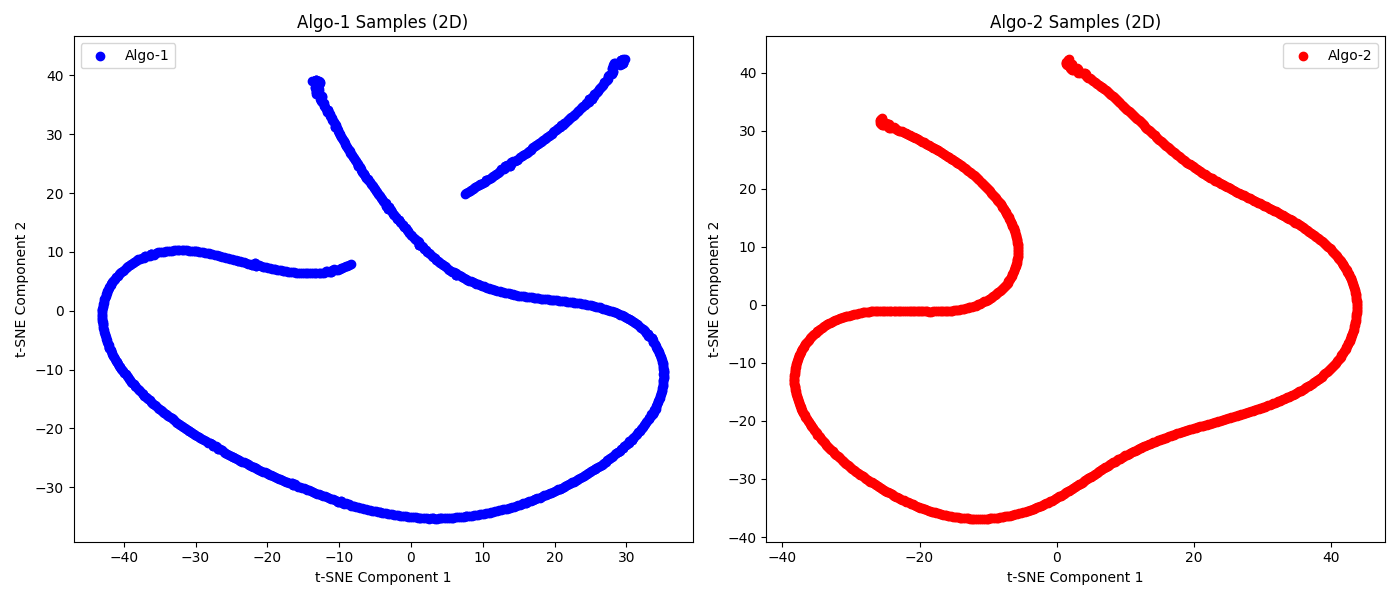
\includegraphics[width=\linewidth]{TASK-0-1/algo_samples_2d.png}
    \caption{2D visualization of generated samples}
    \label{fig:2d_samples}
\end{figure}
\begin{figure}[H]
    \centering
    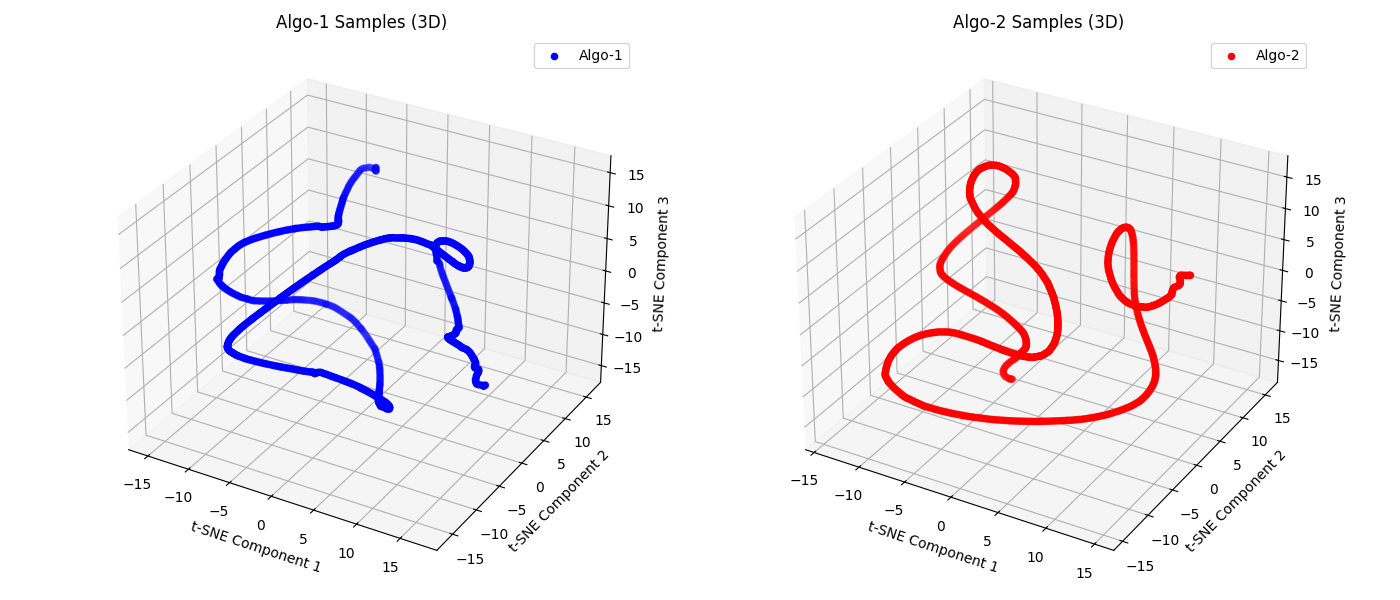
\includegraphics[width=\linewidth]{TASK-0-1/algo_samples_3d.png}
    \caption{3D visualization of generated samples}
    \label{fig:3d_samples}
\end{figure}

\section{Task 2: Approximating Branin-Hoo Using Gaussian Processes}

\subsection{Plots:}

\subsubsection{EI:}
\figrow{EI}{10}{rbf}
\figrow{EI}{10}{matern}
\figrowescaped{EI}{10}{rational_quadratic}
\figrow{EI}{20}{rbf}
\figrow{EI}{20}{matern}
\figrowescaped{EI}{20}{rational_quadratic}
\figrow{EI}{50}{rbf}
\figrow{EI}{50}{matern}
\figrowescaped{EI}{50}{rational_quadratic}
\figrow{EI}{100}{rbf}
\figrow{EI}{100}{matern}
\figrowescaped{EI}{100}{rational_quadratic}

\subsubsection{PI:}
\figrow{PI}{10}{rbf}
\figrow{PI}{10}{matern}
\figrowescaped{PI}{10}{rational_quadratic}
\figrow{PI}{20}{rbf}
\figrow{PI}{20}{matern}
\figrowescaped{PI}{20}{rational_quadratic}
\figrow{PI}{50}{rbf}
\figrow{PI}{50}{matern}
\figrowescaped{PI}{50}{rational_quadratic}
\figrow{PI}{100}{rbf}
\figrow{PI}{100}{matern}
\figrowescaped{PI}{100}{rational_quadratic}

\subsubsection{Random:}
\figrow{Random}{10}{rbf}
\figrow{Random}{10}{matern}
\figrowescaped{Random}{10}{rational_quadratic}
\figrow{Random}{20}{rbf}
\figrow{Random}{20}{matern}
\figrowescaped{Random}{20}{rational_quadratic}
\figrow{Random}{50}{rbf}
\figrow{Random}{50}{matern}
\figrowescaped{Random}{50}{rational_quadratic}
\figrow{Random}{100}{rbf}
\figrow{Random}{100}{matern}
\figrowescaped{Random}{100}{rational_quadratic}

\subsection{Analysis and Comparison:}
\subsubsection{Impact of Sample Size}
The performance of Gaussian Process (GP) models is directly proportional to the amount of available training data. As the sample size increases, the model gains more information about the black-box function, which reduces its predictive uncertainty. This is evident in the decreasing standard deviation across the input space. With more data, the GP has better coverage of the domain, allowing it to interpolate with greater confidence and capture complex function behavior more accurately.

At 100 samples, the predicted mean closely resembles the structure of the true Branin-Hoo function and exhibits smoother transitions and finer detail, especially near function minima. The reduction in uncertainty is due to having more data and also reflects the GP's probabilistic nature, where confidence grows as it observes more consistent patterns.

\subsubsection{Influence of Kernel Choice}
The kernel (or covariance function) defines the assumptions a GP makes about the smoothness and structure of the function being modeled.

The RBF kernel leads to very smooth and confident predictions with large sample sizes. Its infinite differentiability assumption makes it useful for modeling functions that are known to be smooth, like Branin-Hoo. This is why at 100 samples, RBF shows very low uncertainty across the domain.

RBF's smoothness assumption can be a problem when data is scarce. It tends to overgeneralize, leading to overconfident predictions in regions far from observed data. On the other hand, Matérn and Rational Quadratic kernels allow for more flexibility and less smoothness and are therefore better for scenarios with fewer samples. They preserve local uncertainty, which can prevent misleadingly confident predictions in undersampled areas.

\subsubsection{Understanding Uncertainty and Model Confidence}
One of the advantages of GPs is their ability to quantify uncertainty. This feature is important in active learning and optimization settings where decisions about where to sample next depend on the predicted values and on the model’s confidence.

At low sample sizes, uncertainty is high across most of the input domain. This is expected given the limited observations. The only exceptions are near training points, where the model has direct evidence and can make accurate predictions. As more data is added, this uncertainty reduces. \\ \\
Note: If the kernel has a strong bias (RBF has a tendency to oversmooth), not all low-uncertainty regions imply correctness.

\subsubsection{Performance of Acquisition Strategies}
Acquisition functions in Bayesian optimization provide a non-deterministic method for selecting the next best sample point. They attempt to balance uncertainty reduction and refining promising areas.

EI generally proves more effective because it considers both the mean and variance of the GP prediction, guiding the search toward regions that are uncertain and potentially optimal. This balance is important when the global optimum lies in an undersampled area.

PI focuses on improving the best current prediction. While this can lead to faster improvements initially, it may ignore unexplored regions, increasing the chance of getting stuck in local optima, especially when the GP’s uncertainty is underestimated.

These strategies work best when the sample size is small, as they make intelligent use of limited data. As the model becomes more confident with larger datasets, the relative impact of the acquisition function reduces, though EI still performs better in convergence efficiency.

\subsubsection{Conclusion}
With a large enough dataset, rigid kernels like RBF perform well, but under limited data, more adaptable kernels and intelligent acquisition functions make a big difference. The takeaway is that Bayesian optimization is very powerful when uncertainty is correctly estimated and intelligently used. 

\section{Individual Contributions:}
All 3 team members made significant contributions to the assignment.
\begin{itemize}
    \item Tejas Sharma: Task 0,1
    \item Muskaan Jain: Task 2 Code and Analysis
    \item Ojas Maheshwari: Task 2 Analysis
\end{itemize}

\section{Sources:}
\begin{itemize}
    \item Task 0,1: ChatGPT for plotting and understanding TSNE from SkLearn.
    \item Task 2: ChatGPT for Python array dimensions and small fixes. The algorithm was coded from scratch, referring to the class slides. AI assistance for understanding the exact use and implications of different kernels and acquisition strategies. 
\end{itemize}


\end{document}
